\chapter{Background}
\label{chapt:bg}
\section{Algorithm Overview}
\label{agloover}
Ant Colony Optimisation is a probabilistic technique usually used on problems which can be resolved by returning an optimal path through a graphical representation of a given problem. Ant Colony Optimisation refers to a collection of methods and techniques which represent a specific family in Swarm Intelligence. Swarm Intelligence \enquote{...deals with natural and artificial systems composed of many individuals that coordinate using decentralized control and self-organization. In particular, the discipline focuses on the collective behaviours that result from the local interactions of the individuals with each other and with their environment} \cite{SI:def}. In summary each agent is simple and follows a series of basic rules as it performs its operations. If you increase the population of these agents and allow them to communicate with each other then the world they populate will express an emergence of intelligence otherwise unavailable to any individual agent. Ultimately each agent collectively works towards the same goal increasing the quality and appropriateness of the result.

Ant Colony Optimisation algorithms stemmed from the initial proposal by Marco Dorigo et al. through the publication of his PhD in 1992 \cite{Dor1992:thesis}. The Algorithms are based upon the real world behaviour of ant colonies. Ants in the real world will generally always find the most optimal bath between two or more locations, often described as the route between their nest site and the location of the food source(s). As an ant leaves the colony in search of a food source it begins to deposit a chemical trail (pheromone) which can be analysed by other ants in the population. Once an agent has deposited the pheromone it starts to decay. This decay rate could be accelerated by external factors such as adverse weather conditions or movements in the terrain. As the pheromone decays, new pheromone will be deposited by other agents in the colony. As more and more agents continue their tour the locations which have the highest concentration of pheromone are generally the most traversed locations. Ultimately the locations with the highest concentration of pheromone will not only be the most frequently used but will also form the optimal route between the start location and the destination(s). Every location is subject to such decay however the most commonly used locations will constantly be ‘topped up’ by the population whereas the locations used less frequent will ultimately decay to low pheromone levels. The pheromone levels are important because they directly influence the probabilistic function for any ant choosing its next location at any intersection. The higher the concentration of pheromone, the greater the probability that the ant will choose this location as the next stop on its tour. As this is a probabilistic decision the ant may not always choose the location with the highest concentration levels allowing for other solutions to be sought after, enabling shifts in the current best route.

\section{Double Bridge Experiment}
\label{dblbridge}
The double bridge experiment is an early experiment devised to help understand the real world behaviour of ants and their path finding capabilities. The double bridge experiment, as the name suggests involves a nest location separated from a single food source by two bridges. This experiment was designed and carried out by Deneubourg and colleagues in 1989-1990 and used real Argentine ants \cite{marcdorgio:book:doublebridges}.

\begin{figure}[h!]
\centering
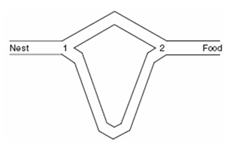
\includegraphics[width=0.5\textwidth]{Images/chapter1/doublebridge}
\caption[Double Bridge Experiment]{Image representing the Double Bridge Experiment. Image source \cite{doublebridges:image}}
\label{fig:doublebridge}
\end{figure}

\noindent
Figure \ref{fig:doublebridge} represents the scenario the Argentine ant were faced with for the Double Bridge Experiment. Initially there will be no pheromone trails for the ants to follow, so as the first ant approaches intersection marked \enquote{1} in figure \ref{fig:doublebridge} the probability that they choose the top path, or lower path is therefore $\approx$50\%. Regardless of which path the ant chose pheromone will now be deposited on the corresponding path. The next ant will approach the intersection marked \enquote{1} however, as there now exists a pheromone trail this ant now no longer has an equal probability to choose either path but instead is more likely to choose the same path as the previous ant. This process will continue for every ant in the colony. Generally speaking as the bottom path is significantly longer than the top path, the pheromone deposited on the lower path will ultimately have a lower pheromone concentration than the shorter top path. Overtime this will cause more and more ants to take the top path over the bottom path due to the higher pheromone level directly impacting the probability of the ant choosing this path. The same applies to intersection marked \enquote{2}, the ants will still tend to prefer the path with the greater pheromone concentration, the fact that the ant now has food does not affect the ants choice in anyway, aside from the fact that the ants new target is the nest and no longer the food source.

\section{Travelling Salesman Problem}
\label{tsp}
Ant Colony algorithms are commonly applied to the Travelling Salesman Problem (TSP). The TSP consists of a graph of $n$ cities and a path between these $n$ cities must be found however, each city must be visited exactly once. Generally this $n$ value is rather large for example the Berlin52\cite{berlin52:source} is a variation of the TSP where this $n$ value is 52. The number of possible routes between these 52 cities is incredibly large. The application of heuristic algorithms such as the Ant Colony methods enables solutions to be found within a reasonable time. One solution for the Berlin52.tsp problem is shown in figure \ref{fig:berlin52}.

\begin{figure}[h!]
\centering
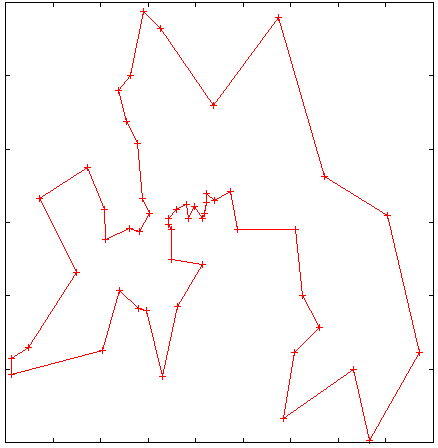
\includegraphics[scale=0.7]{Images/chapter1/tsp52}
\caption[Example Berlin52.tsp Solution]{One solution to the Berlin52.tsp problem plotted using GNU Plot. Modified version from original image source \cite{berlin52:image}}
\label{fig:berlin52}
\end{figure}

The TSP is not the only problem which can be tackled using the Ant Colony family of methods. As these methods have metaheuristic properties the general behaviours and structure can be applied to several other problems such as image segmentation however, this project will not cover such problems and will focus on the TSP style of problem.

\section{Ant System}
\label{sec:AntSystem}
The Ant System is the most basic implementation of an Ant Colony Optimisation method, because of this it provides the basis for extensions and variations. Due to its basic nature, the Ant System is ideal for demonstrating and teaching the behaviours of a virtual ant colony to a user, and it can be done regardless of their prior background knowledge. In this implementation there is no recollection of the best path between iterations and every agent is equal in terms of its importance in finding a solution.

\subsection{Forumlae}

Sections \ref{ASprob} and \ref{ASphero} refer to the underlying formulae which govern the agents pheromone deposits for a given edge and the probability for an agent to move to a specific location from its current one.

\subsubsection{Probability}

The probability formula is as described in appendix B section \ref{sssec:probfuncsssec}. This is the function which drives the agents movements and enabled agents to generally pick the best looking path (path with the strongest pheromone concentration) whilst also allowing for agents to select other paths helping to prevent localised solutions forming.

\label{ASprob}

\subsubsection{pheromone}

The pheromone function for the Ant System algorithm is as described in appendix B, section \ref{sssec:pherodepo}. This function is the main difference between the Ant System implementation and the Elitist Ant System.

\label{ASphero}

\section{Elitist Ant System}
\label{eliteymcneaty}
The Elitist Ant System is the first adaptation to the initial Ant System algorithm. The Elitist Ant System is again, proposed by Marco Dorgio et al. in his 1992 PhD Thesis \cite{Dor1992:thesis}. The main difference between the Elitist Ant System and the Ant System is the fact that the best ants for a given iteration have pheromone deposited upon their route. This means that the best $x$ number of ants where $x$ is an integer representing the number of elite ants will have their routes remembered across iterations preserving their best routes knowledge. This generally improves performance of the population as a whole as the extra pheromone on these elite paths will increase the probability that any agent traverses an elite edge (an edge that is part of a best routes).

\subsection{Forumlae}

Sections \ref{EASprob} and \ref{EASphero} refer to the underlying formulae which govern the agents pheromone deposits for a given edge and the probability for an agent to move to a specific location any time it reaches an intersection.

\subsubsection{Probability}
\label{EASprob}

The probability function for the Elitist Ant System remains the same as it is in the Ant System, see section \ref{ASprob} and appendix B, section \ref{sssec:pherodepo}

\subsubsection{pheromone}
\label{EASphero}
The pheromone function used in the Elite Ant System takes into account that there is pheromone to be deposited along the current $x$ elite routes.

\begin{figure}[H]
\Large
\begin{equation}
p_{xy}^{k} = (1 - \rho)\tau_{xy}^{k} + \Delta\tau_{xy}^{k} + e\Delta\tau_{xy}^{best}
\end{equation}

\caption[Elitist Ant System Pheromone Function]{Algebraic model of the pheromone deposit function for the Elitist Ant System \cite{marcdorgio:book:EAS}}
\label{fig:EASpheromonefunc}

\end{figure}

The majority of the formula remains the same as defined in appendix B section \ref{sssec:pherodepo} however, there is the addition $e\Delta\tau_{xy}^{best}$. This is the part of the formula which is responsible for the pheromone deposit on current the retained best (elite) paths. $xy$ refers to the $x$ and $y$ coordinate for an edge in the best path this is where pheromone will be deposited. $best$ simply donates that this edge belongs to one of the currently stored best paths. The $e$ value is a constant, and varies between implementations. Research suggests that a good value for this constant, $e$ is $\frac{1}{4}\ .\ \#\ of \ nodes$ \cite{sjored:Thesus2012:evalue} however, there is evidence to support using $\#\ of \ nodes$ as the $e$ value\cite{marcdorgio:book:nopage}.

\section{Existing Solutions}
\label{existingsolutions}
There are a number of pre-existing solutions which attempt visualise Ant Colony algorithms however, the majority of these based upon the authors experience are in fact sub-par in performance. Rather that visualising the algorithms execution in a logical manner, more often than not the existing solutions simply show the algorithms final state l without any detailed intermittent steps. This leaves the author confused about what has just actually happened and how was such a solution obtained.

Another problem associated with existing solutions is that the graphical user interface is too cluttered or complex. Many of the existing applications the author observed contained every interaction element in a tightly packed series of containers rather than splitting appropriate actions into separate views or menus. This is extremely confusing and makes it difficult to actually use the application as intended. If the user has selected that they want to use a specific variation of an Ant Colony algorithm then the user should only be able to interact with the features directly relevant to their selection.

One of the major problems the author faced when assessing the competition was the fact that there was rarely any visualisation of the agents themselves. As a result the user had to effectively guess which cities the agents were currently at. In addition to this there was no visualisation of the agent’s movement between city locations. This made it difficult to visualise the path the agents took aside from coming to your own conclusion based on the pheromone trails which were also often poorly represented.

\section{User Interaction Methods}
\label{uiMethods}
As discussed in section \ref{existingsolutions} the methods of user interaction must be superior to what is provided by the competition. This application will be authored in accordance with several preferred user interaction methods enabling a more user friendly experience for all users and not just those who are experienced with this or similar applications.

\subsection{Law of Context}

The law of context refers to the users expectation that they should only see interface controls relevant to the current object they want to modify \cite{99designs:laws}. This relates to one of the fundamental problems found in competitor applications (see section \ref{existingsolutions}). Should the user request a change of algorithm type which requires an extension to default features, these new controls will be self-contained and represented suitably so the user knows that the new dialogues or interaction methods are a direct result of a change in algorithm type.

\subsection{Law of Feedback}

The law of feedback relates the ideology that every significant action has some form of informative, relative feedback associated with it\cite{99designs:laws}. This enables the users to quickly develop an understanding of what interaction control which action. This also covers any incorrect actions performed by the user. The application will be developed in such a way that any incorrect actions will be displayed to the user in a manner that anyone can understand and provide the user with the required knowledge to resolve said issue.

\subsection{Law of Easing}

The law of easing is very important, especially for this application. This law suggests that complex actions should be segmented into simpler steps to allow the user to comprehend what they are actually doing \cite{99designs:laws}. The way this application will adopt this is that rather than specifying all of the algorithm’s parameters at once, each parameter will have its own method of interaction and its own series of user feedback prompts enabling any user to simply modify select parameters however they see fit, assuming the value is legal.

